\chapter{Methodology and Activities}

\section{Methodology}
The methodology utilized to bring CampusFlow to life involved an agile Software Development Life Cycle (SDLC). The primary focus was on developing a comprehensive, native-feeling mobile application with an intuitive User Interface (UI) and a highly scalable, real-time backend architecture. Recognizing the hardware constraints of average student smartphones, extreme care was taken to prevent the app from becoming bloated or storage-heavy. To achieve this, a NoSQL cloud database was utilized to manage real-time data synchronization efficiently, and lightweight third-party APIs were integrated to offload heavy processes like image hosting to external servers.

\section{Activities Conducted: The Four Core Modules}
The primary engineering activity was designing, coding, and thoroughly testing the four core modules of the CampusFlow ecosystem. Each module was built to solve a specific pain point identified during the community study.

\subsection{Module 1: Lost \& Found Hub}
This module acts as a digital campus noticeboard specifically for lost assets. Users can easily upload details, locations, and images of lost or found items, complete with distinct color-coded tagging (e.g., "Red" for Lost, "Green" for Found). This module drastically reduces the time it takes to match a lost item with its rightful owner.

\begin{figure}[htbp]
\centering
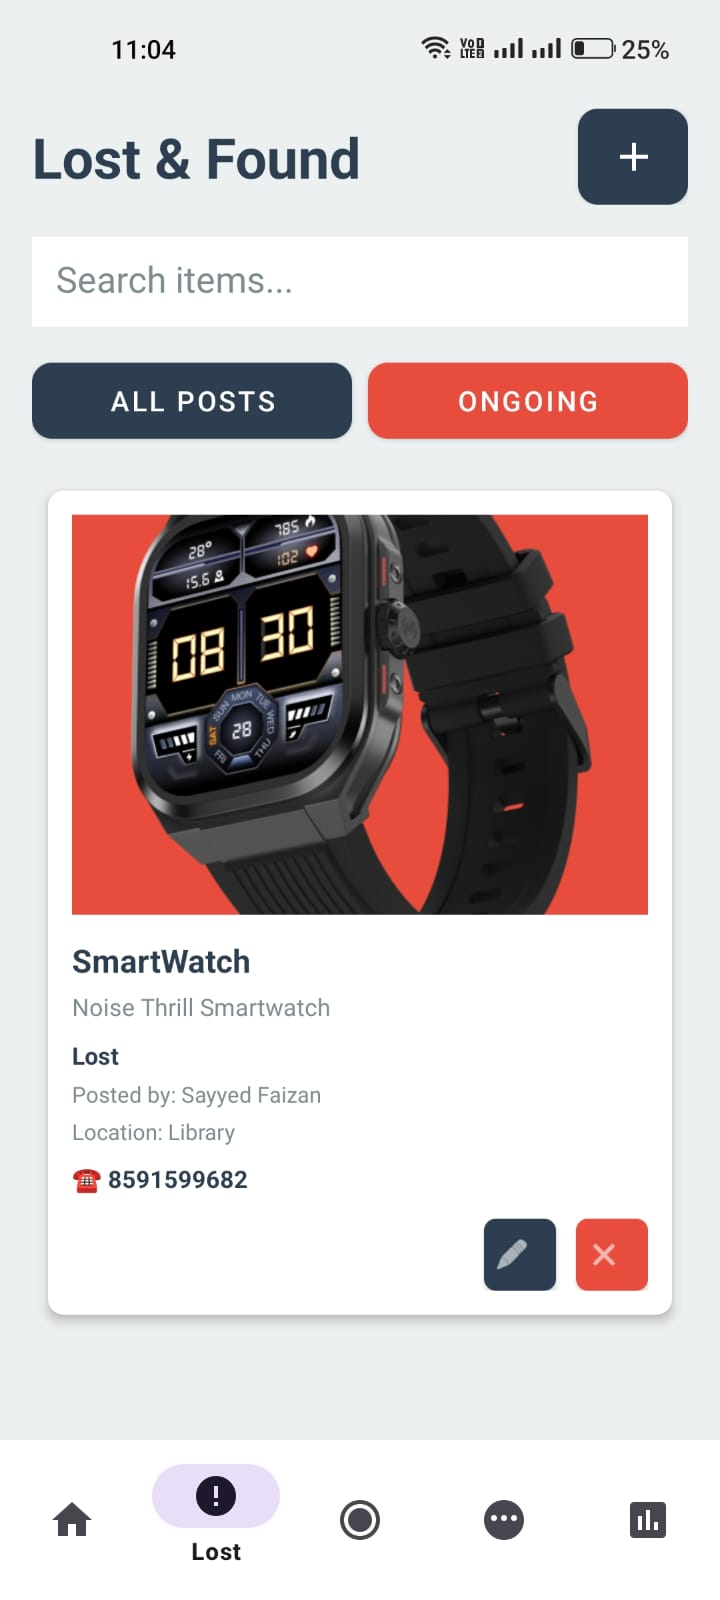
\includegraphics[width=0.4\textwidth]{images/lost_found.png}
\caption{User Interface of the Lost \& Found Module}
\label{fig:module_lost}
\end{figure}

\subsection{Module 2: Project Collaboration \& Networking}
Designed to foster innovation, this hub allows students to post detailed project ideas, specify the technical frameworks they intend to use, and actively recruit team members. It features an inbuilt, real-time chatting system, allowing interested peers to connect instantly and discuss project scopes without needing to exchange phone numbers immediately.

\begin{figure}[htbp]
\centering
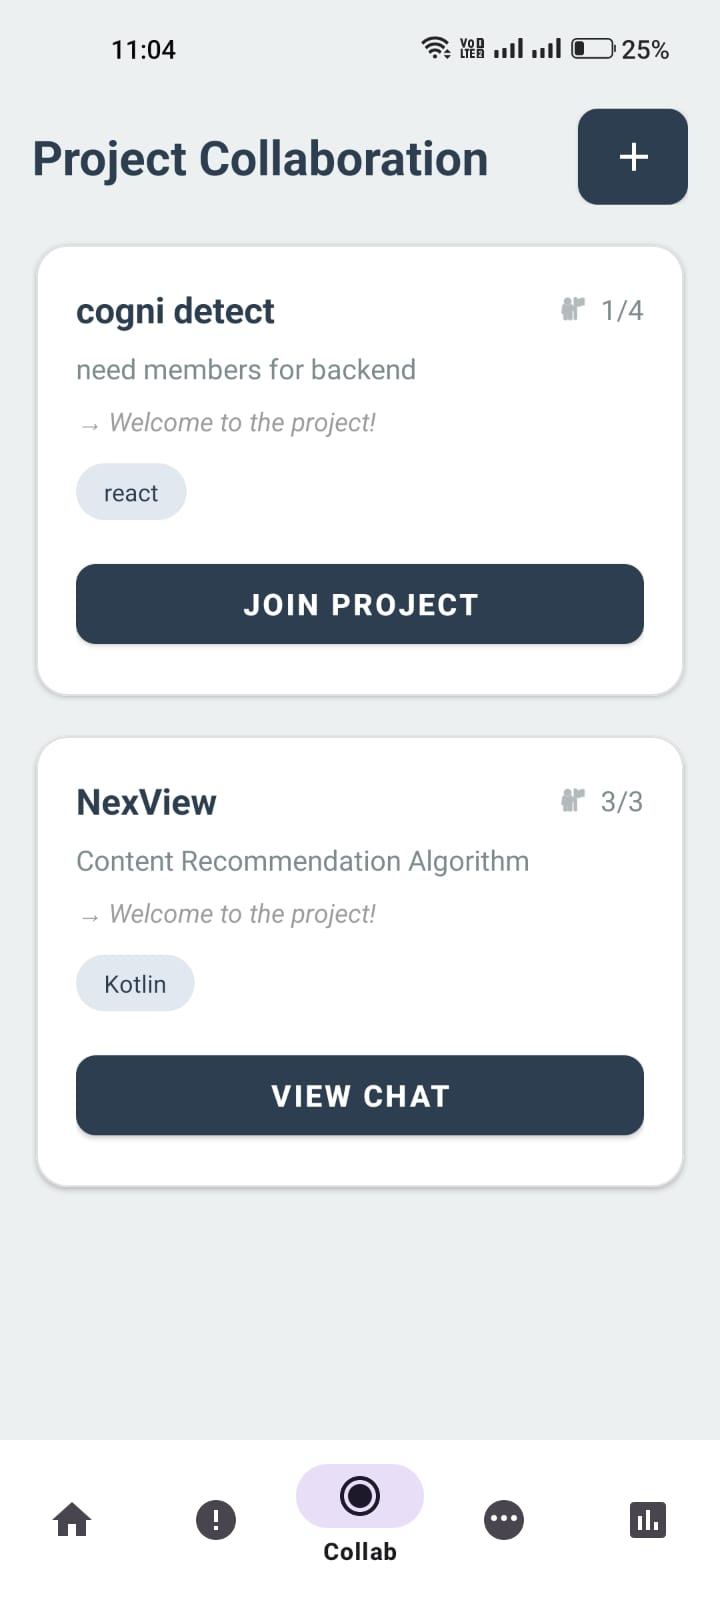
\includegraphics[width=0.4\textwidth]{images/collab.png}
\caption{Project Collaboration Hub and Real-Time Chat Interface}
\label{fig:module_collab}
\end{figure}

\subsection{Module 3: Verified PYQ Repository}
To combat the spread of incorrect study materials, this module serves as a secure, categorized archive for exam preparation. Crucially, upload access is restricted strictly to administrators and verified faculty/student coordinators. This stringent quality control ensures that when a student downloads a document, they can trust its accuracy.

\begin{figure}[htbp]
\centering
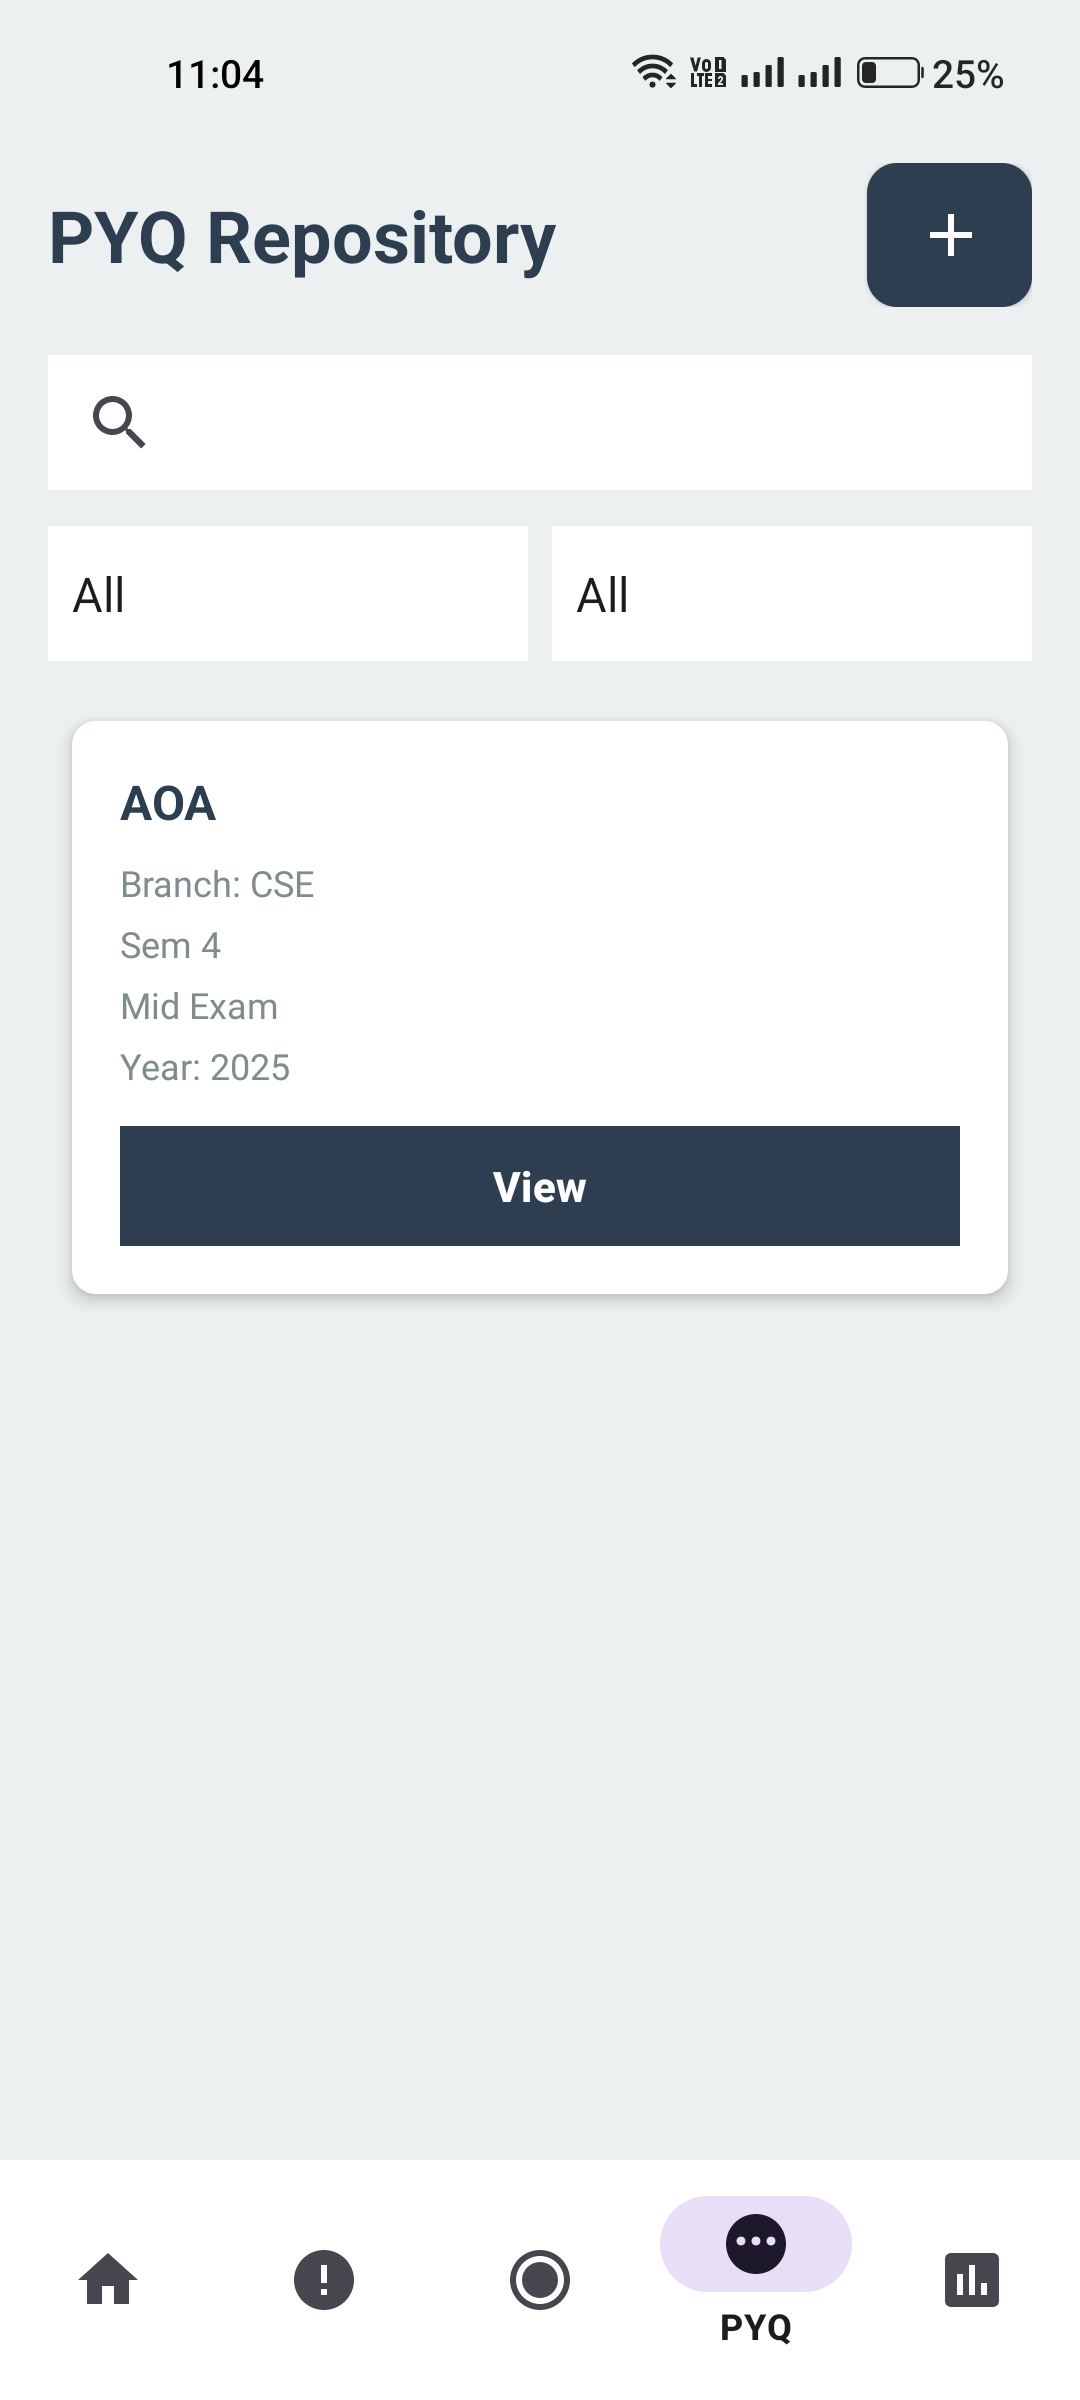
\includegraphics[width=0.4\textwidth]{images/pyq.png}
\caption{Categorized Previous Year Question (PYQ) Repository}
\label{fig:module_pyq}
\end{figure}

\subsection{Module 4: Unified Event Calendar}
This dynamic calendar highlights all upcoming campus events, guest lectures, and hackathons. Maintained exclusively by verified club organizers with admin rights, it ensures students have a single, reliable source of truth for campus activities, effectively eliminating FOMO.

\begin{figure}[htbp]
\centering
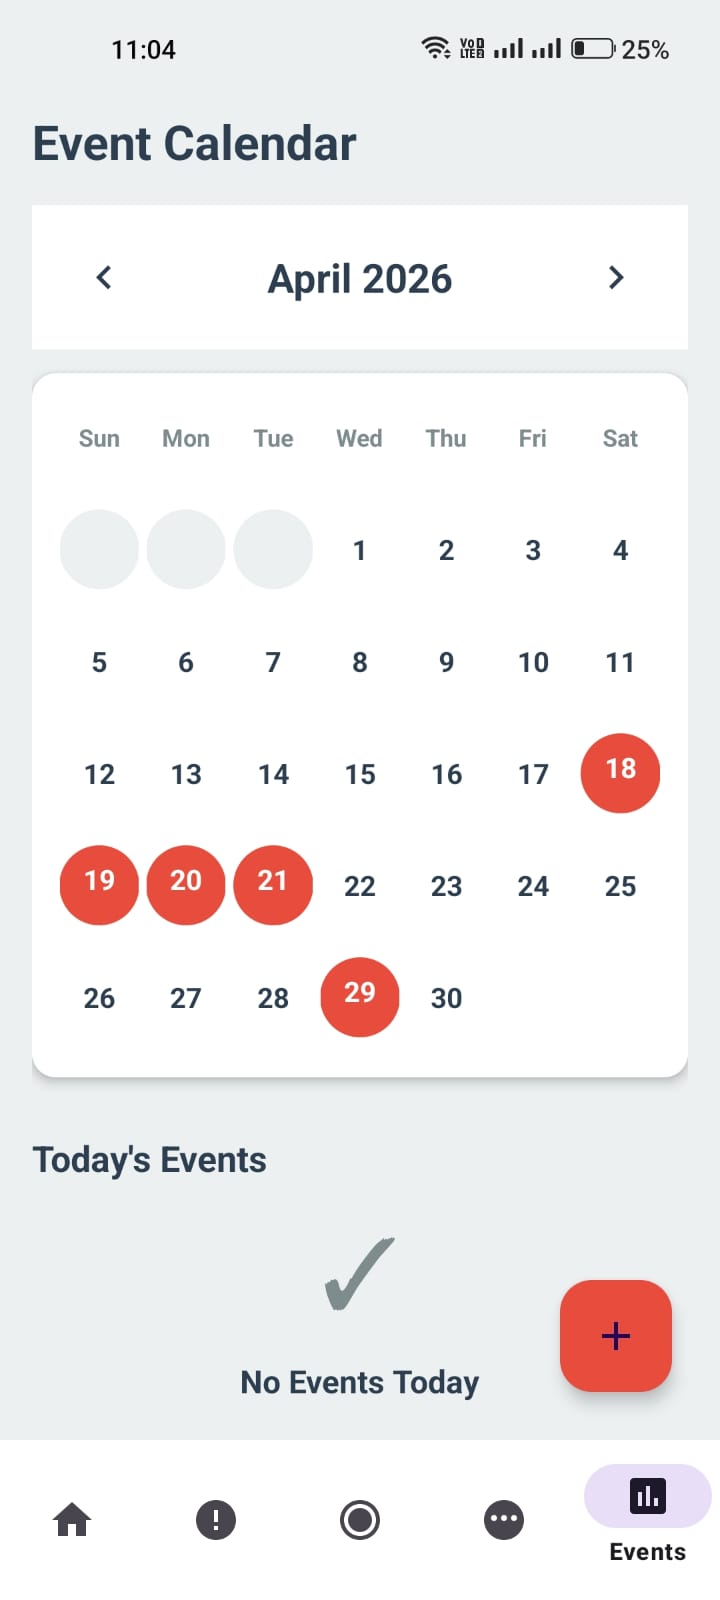
\includegraphics[width=0.4\textwidth]{images/events.png}
\caption{Dynamic Campus Event Calendar}
\label{fig:module_event}
\end{figure}

\section{Tools and Resources Used}
The successful deployment of CampusFlow relied on a carefully curated stack of modern web and mobile technologies, chosen for their performance and cost-efficiency. Table \ref{tab:tech_stack} details the specific technologies implemented.

\begin{table}[htbp]
\centering
\renewcommand{\arraystretch}{1.5}
\begin{tabular}{|p{0.25\textwidth}|p{0.25\textwidth}|p{0.4\textwidth}|}
\hline
\textbf{Architecture Layer} & \textbf{Technology Used} & \textbf{Justification for Selection} \\ \hline
\textbf{Frontend Design} & XML (Extensible Markup Language) & Used to design highly intuitive, responsive, and user-friendly mobile interfaces that adapt to various screen sizes. \\ \hline
\textbf{Core Backend Logic} & Java & Powers the robust core business logic, ensuring smooth app performance and memory management on Android devices. \\ \hline
\textbf{Real-Time Database} & Firebase Firestore & A globally distributed NoSQL cloud database ensuring instantaneous live updates for the chatting and feed features. \\ \hline
\textbf{Media Hosting API} & ImageBB API & Utilized for seamless, lightweight image hosting, highly crucial for optimizing storage space in the Lost \& Found module. \\ \hline
\end{tabular}
\caption{Detailed Summary of the Technology Stack Utilized for CampusFlow}
\label{tab:tech_stack}
\end{table}

Additionally, awareness programs and brief campus-wide training sessions are continuously planned to rapidly onboard campus clubs, faculty members, and the general student body to ensure high adoption rates.